\documentclass[11pt]{article}
\usepackage{graphicx}
\begin{document}
Documentation

\begin{flushleft}
\item 2.1.1 System Interfaces.\newline
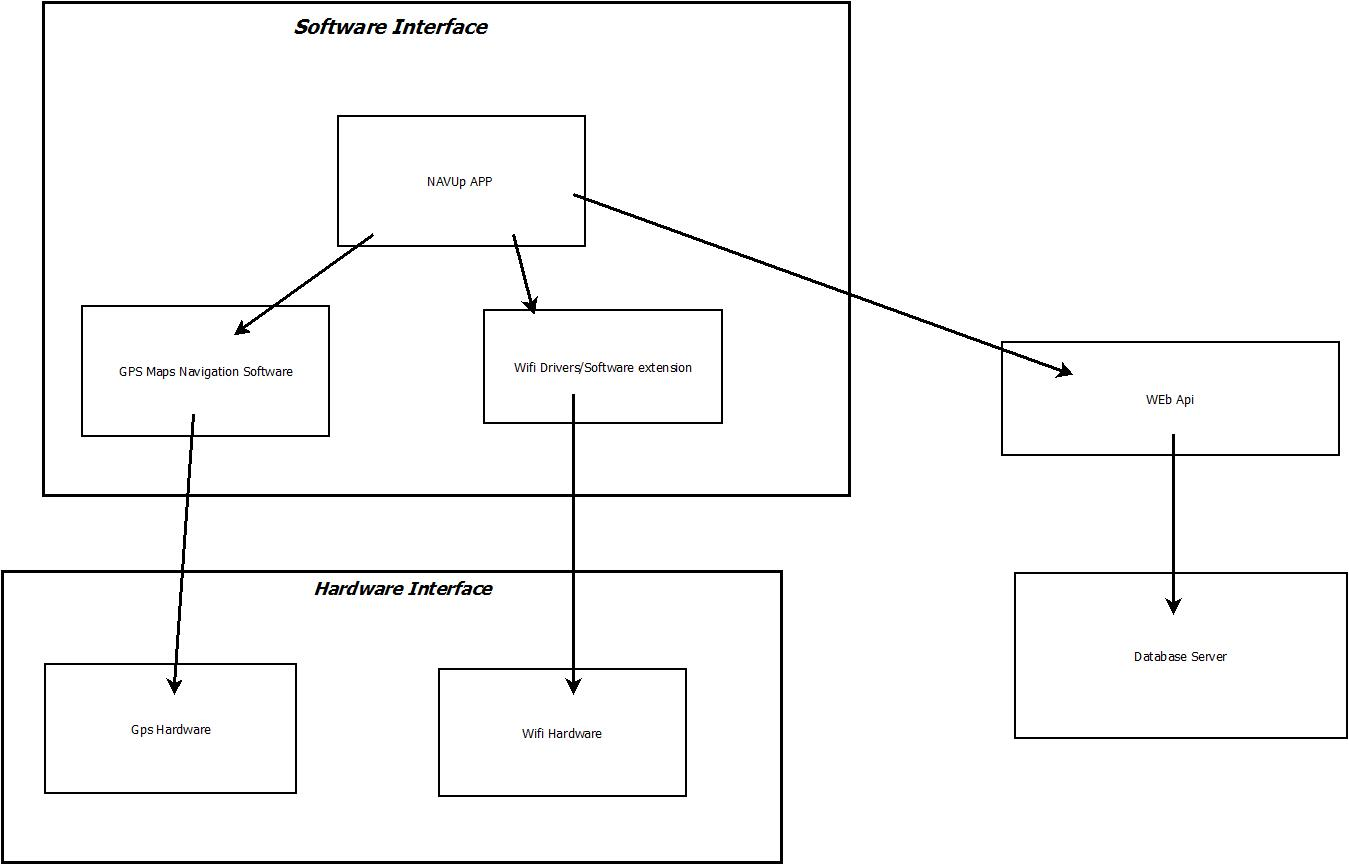
\includegraphics[scale=.5]{SystemInterfaces}
\newline
1.\textbf {Mobile Software Interface} , for full functionality the mobile application requires the Mobile Software interface which contains firstly our Mobile app which is our Web, Android and iOS application, then the GPS mapping software which includes navigation and maps, then lastly in the mobile software interface we have the wifi software extension library that we will use to pin point users locations based on the data from the routers that they are connected to.
\\
2.\textbf{Mobile Hardware Interface}, the hardware interface required for this system is a gps device required by the mapping and navigation software, and the device should have basic wifi connectivity hardware.
\\
3.\textbf{Web Api}, the web api or web server that will be used to pull from the database, do validation and crud information.
 \\
4.\textbf{Database Server},stores all of the users information logs and user details required by NavUp.
\end{flushleft}

\begin{flushleft}
\item 2.1.3 \textbf{Hardware Interfaces }\\
The minimum hardware device required  mainly is a device either cellphone or tablet, that has wifi, gps and internet connectivity with the following device requirements :\\
IPhone 4S, 5, 5C, 5S, 6, 6 Plus, 6S, 6S Plus, SE, 7, or 7 Plus running iOS 8 or later versions\\
For best results: Use iPhone 5 or newer.\\
 Operating System versions Android:\\
Any smart phone from 2013 or newer, running Android version 4.0 or newer\\
For best results: The phone should run Android 5.0 or newer. \\
The application will operate in full screen mode, and will use up an average amount of resoureces,
newer model phones are more likely to perfom beter and are less prone to crashing or freezing.\\
GPS reliability and accuracy: Some low priced phones are known to have GPS connectivity issues. Make sure to Google search “your phone’s model + GPS connectivity” to see its performance specs
More maximum performance.\\
WIFi  reliability: Make sure your device has the minimum wifi hardware needed for a connection to the wifi routers.
\end{flushleft}

\begin{flushleft}
\item 2.1.5 \textbf{Communications Interfaces}\\
This specifies the various interfaces to communications such as local network protocols, etc. The communications interfaces we are using are:\\
1.\textbf{GPS}\\
The GPS network protocols in interaction with NavUp are yet to be determined.\\
2.\textbf{WIFi}\\
The Wifi network protocol in interaction with NavUp are yet to be determined. 
\end{flushleft}

\begin{flushleft}
\item 2.1.7 \textbf{Operations}\\
1.There are four primary operations that can be performed in interaction with the NavUp App:\\
\begin{itemize}
\item Display Users current location\\
\item Searching for locations\\
\item Saving locations and providing directions to a location\\
\item initialise the views, maps and e.t.c\\
\item Different levels of users and agents to enter different types information into the system regarding venues, points of interest, events and activities using multiple types of devices and services.\\
\end{itemize}
These operations will be available to clients by means of appropriate views.\newline


2.These operations can be performed in interaction with the Device Hardware interface:\\
\begin{itemize}
\item open connection to the  wifi network\\ 	
\item open connection to gps network and get current position\\
\item request map interface initialisation data from the device.\\
 \end{itemize}
These operations will be available to clients by means of an appropriate hardware device.\newline

3.These operations  can be performed in interaction with the web Api:\\
\begin{itemize}
\item request user information 	\\
\item request session data\\
\item crud database information \\
\item perform server side processes \\
 \end{itemize}
These operations will be available to NAvUp App by means of an appropriate web connection Protocols.\newline

4.These operations  can be performed in interaction with the database:\\
\begin{itemize}
\item store all required information 	\\
\item communicate with the api \\
 \end{itemize}
These operations will be available to Api by means of an appropriate Database connection Protocols.\\

\end{flushleft}


\end{document}